\chapter{SGSEAM Design}
\label{cha:sgseam-design}

This chapter describes the design of the Serious Game Stakeholder Experience 
Assessment Method (SGSEAM) for assessing serious game frameworks. It starts with the overview of SGSEAM, followed by the discussion of assessment methodology, and the detailed steps of the assessment method. Finally, \autoref {app:sgseam-lucid-guide} illustrates an example of SGSEAM assessment guide written for a specific serious game framework.

\section{Overview}

One of the benefits of using a serious game framework such as Makahiki, is that if correctly designed, it will provide useful and reusable ``building blocks'' with which to develop a variety of serious games. Yet how are we to know if a serious game framework has been ``correctly designed''? As we discussed in the Related Work, there are a few  framework or tools for general purpose assessment of a software system, but I have not yet found any prior work concerning the comprehensive approach for the particular needs of a serious game framework assessment. This is the motivation of the Serious Game Stakeholder Experience 
Assessment Method (SGSEAM). It is designed for assessing serious game frameworks in particular.

Serious Game Stakeholder Experience Assessment Method (SGSEAM) describes a method for 
assessing serious game frameworks from the stakeholder 
experience perspectives.  The goal of SGSEAM is to identify (a) major strengths of a serious game
framework, which aids the community by indicating features of the framework to emulate, and
(b) major shortcomings of the framework, which aids the community by indicating features to avoid.
The benefits of SGSEAM assessment are for the developers of serious game frameworks 
to learn and improve from the findings of the assessment.

The approach that SGSEAM uses is to assess the experiences of various important stakeholders when
they interact with the serious game framework. In the full life cycle of a serious game framework
there are a great variety of potential stakeholders, including:

\begin{itemize}
\item \textbf{Players}: those who participate in the game produced by the framework.
\item \textbf{System admins}: those who install and maintain the technological game infrastructure.
\item \textbf{Game designers}: those who design the content and game mechanics. They include  content experts, instructional designers, etc.
\item \textbf{Game managers}: those who manage the game during the period of game play.
\item \textbf{Game Developers}: those who use the game framework to customize, extend and enhance their games.
\item \textbf{Researchers}: those who are conducting research using the game framework.
\item \textbf{Spectators}: those who do not participate in the game play but are interested in the game and the results of game play. 
\item \textbf{Community partners}: those who partner with the game organizers to help run the game (such as coordinating real-world events as part of the game, providing support for energy data
  collection if the serious game requires energy data, etc) 
\item \textbf{Funding organizations}: the organizations who provide funding for the game or game framework.
\end{itemize}

The scope of SGSEAM is to assess serious game frameworks as software infrastructure. While
the overall success of a serious game depends on the individual success of all of these
stakeholders, SGSEAM only assess the experiences of the players, system admins, game designers, game managers, and game developers, which are closely related to software infrastructure. 

\autoref{fig:sgseam-overview} illustrates the steps of applying SGSEAM to a framework.

\begin{figure}[ht!]
  \center
  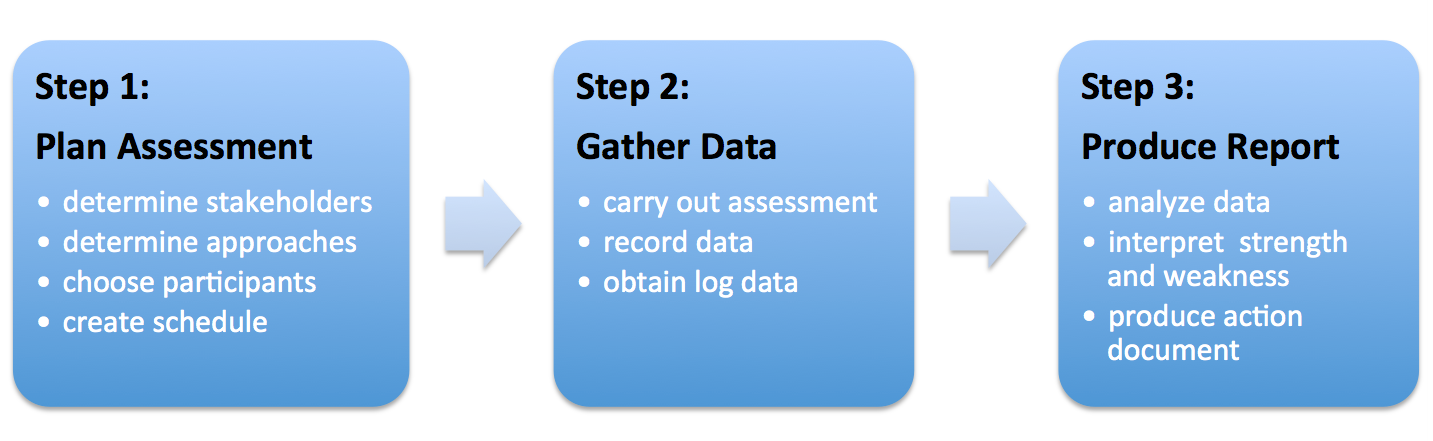
\includegraphics[width=0.9\columnwidth]{sgseam-steps}
  \caption{Applying SGSEAM to a framework}
  \label{fig:sgseam-overview}
\end{figure}

There are three steps in the process of applying SGSEAM:

\begin{enumerate}
\item Step one is to {\bf Plan the assessment}, including
 identifying the stakeholders, determining assessment approaches, and creating the assessment schedule. 
 The deliverable for this step is the \textbf{\textit{assessment
     plan}} document. 

\item Step two is to {\bf Gather data} by carrying out 
 the assessment, recording and obtaining related data. The deliverable for this step is the 
 assessment \textbf{\textit{data repository}}. 

\item Step three is to {\bf Produce the assessment report} by analyzing 
 the data and interpreting strengths and weaknesses. The deliverable
 for this step is the \textbf{\textit{improvement action}} document.

\end{enumerate}
 
The following sections describe the methodology used in SGSEAM, followed by the detailed
description of steps in applying SGSEAM to serious game frameworks.

\section{Methodology}

SGSEAM is an assessment method instead of an evaluation method. The main purpose 
of an evaluation is to determine the quality of a program by formulating a judgment. An assessment, on 
the other hand, is nonjudgmental. SGSEAM does not try to judge a framework according to a 
standard, or to compare one framework against another. Instead, it is used to identify the major 
strengths and shortcomings of a framework to benefit  the developers of the framework.

Creswell \cite{creswell2003} categorizes research methods into three approaches:
quantitative, qualitative, and mixed methods, according to what knowledge claims are being made
and how knowledge is acquired. Quantitative method reflects a post-positivist paradigm where
hypotheses are specified {\em a priori} and tested by experimental design. Qualitative method
reflects a constructivist or participatory paradigm where knowledge would be acquired by
observation and open-ended design. SGSEAM employs the mixed methods approach which based on
pragmatic knowledge claims and assumption that collecting diverse types of data provides better
understanding of the research problem: assessing the strengths and shortcomings of a serious game
framework.

In SGSEAM, the concurrent triangulation strategy described in Creswell's mixed method approach
is used.  Data collection and analysis involves both quantitative information (instrument and
analytical data recorded by the system such as website logs, interaction database, etc), as well
as qualitative information (interviews and questionnaire responses).

SGSEAM follows closely with the "Goal-Question-Metric" (GQM) approach \cite{caldiera1994goal} in
software engineering research. GQM defines a software  measurement model on three levels: a goal
of the measurement, a set of questions to assess the goal, and a set of metrics associated with
each question. There are many metrics related to user experiences \cite{tullis2010measuring}, SGSEAM
focus on the metrics that is useful to provide insights about the strengths and weaknesses of a serious
game framework.

In SGSEAM, the assessment goals are the experiences of the identified stakeholders. For each
stakeholder, a set of questions is used to assess the strengths and shortcomings from the
stakeholder's perspective. For each question, a set of alternative assessment approaches is
described.

\section{Plan the Assessment}

This is the first step of SGSEAM. It first identifies the stakeholders, determines the appropriate assessment approaches according to the available resources, and creates the assessment schedule. The deliverable for this step is the assessment plan document which includes the details of stakeholders, approaches and schedule.

\subsection{Identify stakeholders}

SGSEAM assesses the experiences for the stakeholders listed in \autoref{table:stakeholders}. 

\begin{table}[ht!]
  \centering
  \begin{tabular}{|p{0.2\columnwidth}|p{0.4\columnwidth}|p{0.3\columnwidth}|}
    \hline
    \tabhead{Stakeholder class} &
    \tabhead{Definition} &
    \tabhead{Examples} \\
    \hline
    Player &
    participate in the game produced by the framework. &
    students, residents \\
    \hline
    System admin &
    install and maintain the technological game infrastructure. &
    system admin, IT staffs \\
    \hline
    Game designer &
    design the content and game mechanics. &
    instructional designers, content experts \\
    \hline
    Game manager &
    manage the game during the period of game play.&
    sustainability coordinators, residential staffs\\
    \hline
    Game developer &
    develop customization, extend and enhance the game. &
    programmers, internal developers \\
    \hline
  \end{tabular}
  \caption{SGSEAM Stakeholders}
  \label{table:stakeholders}
\end{table}

For each stakeholder, identify the population, the name and contact if possible. For example, the 
player stakeholder could be identified as the users interact with the game interface, perform certain tasks given by the interface, or winning the prize. The system admins install, backup, monitor the software system. The game designers create the content for the game and design what game mechanics to used. The game managers manage the game during the game period. Finally the game developers develop enhancement and customization using APIs provided by the framework.

It is important to be able to contact the stakeholders in some way, either via email or phone, to get the feedback from their experiences with the framework.

\subsection{Determine assessment approach}

There are usually multiple assessment approaches for each stakeholder.  \autoref{table:approaches} provides 
an overview of the assessment method and the approaches. The appropriate assessment approaches should 
be determined according to the resource available. The approaches for a stakeholder is additive. The more 
approaches applied, the higher confidence of the assessment can be achieved.

\begin{table}[ht!]
  \centering
  \begin{tabular}{|p{0.175\columnwidth}|p{0.3\columnwidth}|p{0.43\columnwidth}|}
    \hline
    \tabhead{Stakeholder}&
    \tabhead{Assessment goal}&
    \tabhead{Assessment approaches} \\
    \hline
    Player&
    Determine the extent the framework affect and engage players.&
    	Pre-post effectiveness study(\ref{Pre-Post effectiveness study});\newline
	Self-reported usability metrics(\ref{Self-reported usability metrics});\newline
	Engagement metrics(\ref{Engagement metrics}) \\
    \hline
    System admin&
    Determine strengths and weaknesses in system install and maintenance.&
    	Post-hoc admin interview(\ref{Post-hoc system admin interview});\newline
	In-lab system admin study(\ref{In-lab system admin study}) \\
    \hline
    Game designer&
    Determine strengths and weaknesses in facilitating the game design process.&
    	Post-hoc designer interview(\ref{Post-hoc game designer interview});\newline
	Game design log data analysis(\ref{Game design log data analysis});\newline
	In-lab game design study(\ref{In-lab game design study})\\
    \hline
    Game manager&
    Determine strengths and weaknesses in managing the game.&
    	Post-hoc manager interview(\ref{Post-hoc game manager interview});\newline
	Game management log data analysis(\ref{Game management log data analysis});\newline
	In-lab game management study(\ref{In-lab game management study})\\
    \hline
    Game developer&
    Determine strengths and weaknesses in developing system enhancement.&
    	Post-hoc developer interview(\ref{Post-hoc game developer interview});\newline
	In-lab game development study(\ref{In-lab game development study}) \\
    \hline
  \end{tabular}
  \caption{SGSEAM approaches}
  \label{table:approaches}
\end{table}

The assessment approaches is categorized into in-vivo and in-vitro assessments. The in-vivo approaches, 
such as pre-post test, in-game surveys and post-hoc interviews, assess the real world instance of the game. 
The in-vitro approaches use in-lab experiments in a simulated environment. Different assessment
approaches will have different levels of rigor or validity. For example, the in-lab experiments (in-vitro) can 
enlist several subjects to perform the same pre-defined tasks and collect comparable data in a more 
controlled setting. It is rigor because of the generality achieved from the larger population of
participants under study. On the other hand, in-game surveys or interviews in the in-vivo approach typically 
collect data from different uncontrolled settings with less rigor. But the in-invo data reflect the real world 
interaction between the stakeholders and the framework, thus provides better insights in the real world settings.

The following sections describe in detailed the different approaches for each stakeholder.  Each assessment 
approach describes the goal of the assessment, what data to collect, how to collect the data and how to 
analyze the data to obtain insights about the strengths and weaknesses of the framework from each 
stakeholder's perspective.

\subsubsection{Player Assessment}

The goal of player assessment is to determine the effectiveness of the game
framework from player's perspective. It is essential that a game produced by a serious game
framework could achieve its intended "serious" purpose. The intended purposes of serious games are
always subject specific. For example, the desired effect of a serious game for
energy education and conservation is to increases players' energy literacy and
reduces their energy consumption during (and, hopefully, after) the game. A serious game for
language learning would have a very different desired effect.

\mypar{Pre-Post effectiveness study}
\label{Pre-Post effectiveness study}

We use a quasi-experimental pre-post study to assess the question of the effectiveness of a serious game framework. 

This approach requires users of SGSEAM to first determine a set of domain-specific questions to assess the 
desired effects of their serious game. For example, a set of questionnaires on sustainability literacy, such as 
knowledge of power and energy, is used to assess the effectiveness of a serious game for sustainability education.

Once the domain-specific questionnaires are determined and designed, present this questionnaires as a 
survey to a random selection of the players before the game starts. After the game ends, present the same 
survey to the same players again. Compare the two set of survey response data to study if the game has an 
impact on the players regarding to the survey subjects. The extent of the changes reflected in the survey 
result indicates the degree of effectiveness of the serious game for this subject.

Serious games often engage players with resources of various types (energy, water, waste, etc.). Collect 
these measurements before, during, and after the game in order to acquire evidence regarding the potential 
impact upon player use of these resources.

\mypar{Self-reported usability metrics}
\label{Self-reported usability metrics}

This approach interviews players about their self-reported experiences with the game. Administrate the 
interview through online survey or face-to-face conversation, although we found that online survey is more 
cost effective than face-to-face conversation. If possible, implement the online survey as an activity inside the 
game. For example, the Makahiki serious game framework implements an online survey activity which 
incentivizes players to complete the survey by rewarding game points for the activity.

SGSEAM proposes to use the usability questionnaires outlined in \autoref{fig:usability-metrics} in the online survey or face-to-dace interview:\\

\begin{figure}[ht!]
\begin{mybox}
\begin{compactenum}
\item What did you like most about the game?
\item What did you found confusing?
\item What issues did you have while using the game?
\item What was the thing you liked the least about the game?
\item What can we do to improve the game?
\item It was easy to find what I was looking for on the website.  \\
	Strongly disagree  -  Disagree  -  Neutral  -  Agree  -  Strongly agree
\item The website was responsive. \\
	Strongly disagree  -  Disagree  -  Neutral  -  Agree  -  Strongly agree
\item The website provided adequate help in teaching me how to play. \\
	Strongly disagree  -  Disagree  -  Neutral  -  Agree  -  Strongly agree
\item I understood how to play. \\
	Strongly disagree  -  Disagree  -  Neutral  -  Agree  -  Strongly agree
\item this is something my friends should participate in. \\
	Strongly disagree  -  Disagree  -  Neutral  -  Agree  -  Strongly agree
\end{compactenum}
\end{mybox}
\caption{Player self-reported usability metrics questionnaires}
\label{fig:usability-metrics}  
\end{figure}

\mypar{Engagement metrics}
\label{Engagement metrics}

This approach calculates the engagement metrics to assess the extent of engagement from players and 
the impact of the game. The more engaging the game is, the more potential impact could be to the players.

Player engagement is an important measure for understanding the effectiveness of a serious game.
By investigating the degree of engagement, we can determine to what extent individuals are
participating in the game, as well as to what extent the community population is participating in
the game. On the other hand, engagement has a subtle relationship to the overall effectiveness of a 
serious game. It is possible for the game to be played by only a subset of the target population, but
have an impact on those not playing by virtue of their contacts with players. Gaining
better insight into this diffusion effect could be an interesting research area. 

SGSEAM proposes to calculate as many as possible the player engagement metrics described in \autoref{figure:engagement-metrics} 
by analyzing the data from system log or other channels provided by the framework. The more metrics 
obtained, the better understanding of the extent of player engagement. 

\begin{figure}[ht!]
  \centering
    \begin{tabular}{|p{0.2\columnwidth}|p{0.35\columnwidth}|p{0.35\columnwidth}|}
    \hline
    \tabhead{Metric} &
    \tabhead{Definition} &
    \tabhead{Mesure} \\
    \hline
    participation &
    percentage of players who play the game &
    the level of involvement from players \\
    \hline
    player &
    number of players per day &
    the frequency of players interact with the game \\
    \hline
    play time &
    play time of a player per day &
    the frequency of players interact with the game \\
    \hline
    submission &
    submissions of all player per day &
    the rate of players' completion of game activities \\
    \hline
    social interaction &
    social interaction of all player per day &
    the rate of in-game social interactions between players\\
    \hline
    game error &
    game errors per day &
    the rate of errors encountered by players during the game \\
    \hline
  \end{tabular}
  \caption{Player engagement metrics}
  \label{figure:engagement-metrics}
\end{figure}

The participation rate measures the percentage of users who used the game based on the total
eligible players. In the serious game context, it indicates the level of involvement or awareness
of the serious matters. The number of players and play time per day measure how frequently the
players interact with the game. The submissions per day measures the rate of serious game
specific activities (online or real world) that players completed, while the social interaction
per day measures the rate of social interactions happened in the game between the players. At
last, the website errors per day measures the rate of errors encountered by the players while
using the game website. 

With the exception of the game error metric, the higher value these metrics are, the higher engagement 
level the game has.

\subsubsection{System admin assessment}

System administrators are responsible for installing and maintaining the software infrastructure
for the game. Their tasks include the framework and dependency installation, maintain the database, 
backups, and so forth. The goal of system admin assessment is to determine to what extent the 
framework facilitates the system administration tasks from system admin's perspective. SGSEAM 
assesses how much time is required to install and maintain an instance of a serious game using the 
framework and the problems encountered  during the system admin process.
 
SGSEAM proposes two assessment approaches.

\mypar{Post-hoc admin interview}
\label{Post-hoc system admin interview}

This approach assesses the system admin's experience using the post-hoc interview. The system admins 
are asked about their experience with the framework after they completed the installation and maintanence
 in the production system. The interview questions are described in \autoref{fig:system-admin-interview}.

\begin{figure}[ht!]
\begin{mybox}
\begin{compactenum}
\item How much time did you require to install the system and the dependencies?
\item What problems did you encounter when installing the system and the dependencies?
\item How much time did you require to maintain the system?
\item What problems did you encounter when maintaining the system?
\item Did you find it difficult to admin the system? What was difficult?
\end{compactenum}
\end{mybox}
\caption{System admin interview questionnaires}
\label{fig:system-admin-interview}  
\end{figure}

The interview should be tape-recorded. Once the interview is completed, qualitative data
analysis is performed against the interview data by doing: (1) transcribing the recordings; 
(2) coding (categorizing) the time and problems or difficulties encountered. These data reveal the 
strengths, weaknesses and the areas of improvement for the framework.

\mypar{In-lab system admin study}
\label{In-lab system admin study}

This approach assesses the system admin's experience using the in-lab experimental study. First identify a group 
of participants who have some levels of system administration experience. Second, provide instructions on 
each installation steps, ask the participants to install the system according to the instructions, and ask them to record 
the time spent and problems encountered as they complete each step.

Once the experiment data is collected, categorize the reported problems and correlated with the reported time data 
to identify the areas of strength (less time spent) and weakness (more time spent and problems or difficulties). 

The level of confidence of the above two assessment approaches varies. The experimental study
approach is more rigor because of the generality achieved from the larger population of
participants under study. The data collected during the step by step experimental study is more
accurate than the one collected in the post-hoc interview.

\subsubsection{Game designer assessment}

A game designer uses the serious game framework to design and create a serious game.
A serious game framework normally provides tools or interfaces for game designers
to facilitate the design of a game. For example, the framework provides interface to configure the game period, set up 
players, and tools to design individual game elements.

The goal of SGSEAM game designer assessment is to determine the strengths and weaknesses of the framework 
regarding to the game design process. SGSEAM assesses the game designer stakeholder by addressing the following 
two questions: (a) How much time is required to design an instance of a serious game using the framework? and (b) How
many, and how problematic are the errors that designers encounter during the design process?

There are two approaches for game designer assessment:

\mypar{Post-hoc designer interview}
\label{Post-hoc game designer interview}

This approach interviews the game designer(s) after they had completed the design of a serious game using the 
framework in a production system. The interview includes the questions described in \autoref{fig:game-designer-interview}.
 
\begin{figure}[ht!]
\begin{mybox}
\begin{compactenum}
\item How much time did you spend to complete each design task?
\item What problems did you encounter?
\item Did you find it difficult to configure? What was difficult?
\item Did you find it difficult to design a specific game? Which one, and what was difficult?
\end{compactenum}
\end{mybox}
\caption{Game designer interview questionnaires}
\label{fig:game-designer-interview}  
\end{figure}

The interview should be tape-recorded. After the interview, transcribed the recordings, code and categorize the reported 
time and problems to identify the strengths and weaknesses.

In addition, if possible, collect the system log data related to the game designing tasks, analyze the logs to find out the time 
spent and error encountered during the game designing tasks. Use the log data to verify the findings from the interview data.

\mypar{In-lab game design study}
\label{In-lab game design study}

This approach assesses the game designer experience using the in-lab experimental study.  First identify a group 
of participants who are somewhat familiar with the subject domain of the game. Second, provide instructions on 
each designing steps, ask the participants to design the game according to the instructions, ask them to record 
the time spent and problems encountered as they complete each step.

Once the experiment data is collected, categorize the reported problems and correlated with the reported time data 
to identify the areas of strength (less time spent) and weakness (more time spent and problems or difficulties). 

\mypar{Game design log data analysis}
\label{Game design log data analysis}

This approach collects the system log data related to the game designing tasks. When
available, the time spent and error encountered can be queried from the system logs. Although these
system generated data might be easier to gather in some systems, it might not provide the same
depths or insights than the other two approaches where the experiences are provided by the
participants directly. On the other hand, these system data can be supplemental to the other
approaches. They could be correlated with the data gathered from the other assessment approaches
 to increase the confident of the assessment.

\subsubsection{Game manager assessment}

A game manager uses the serious game framework interface to manage the serious game that the game
designers created. It is possible that a game manager is also the game designer.
The examples of game management tasks includes managing player submissions, monitoring the game 
state, entering manual resource data, notifying winners of the game, etc.

The goal of SGSEAM game manager assessment is to determine the strengths and weakness of the framework 
regarding to the game management process. Similar to the assessment of the game designer, SGSEAM assesses 
the game manager stakeholder on the time it required to manage an instance of a serious game using the framework
and the problems encountered during the managing process.

SGSEAM proposes two approaches for assessment game manager's experience.

\mypar{Post-hoc manager interview}
\label{Post-hoc game manager interview}

This approach interviews the game manager(s) after they had managed a serious game using the framework 
in a production envrionment. The interview questions are described in \autoref{fig:game-manager-interview}.
 
\begin{figure}[ht!]
\begin{mybox}
\begin{compactenum}
\item How much time did you spend to complete each managing task?
\item What problems did you encounter?
\item Did you find it difficult to manage? What was difficult?
\end{compactenum}
\end{mybox}
\caption{Game manager interview questionnaires}
\label{fig:game-manager-interview}  
\end{figure}

The interview should be tape-recorded. After the interview, transcribed the recordings, code and categorize the reported 
time and problems to identify the strengths and weaknesses.

In addition, if possible, collect the system log data related to the game managing tasks, analyze the logs to find out the time 
spent and error encountered during the game managing tasks. Use the log data to verify the findings from the interview data.

\mypar{In-lab game management study}
\label{In-lab game management study}

This approach assess the game manager's experience using the in-lab game management study.  First identify a group 
of participants who are somewhat familiar with the subject domain of the game. Second, provide instructions on 
each managing tasks, ask the participants to complete the tasks following the instructions, ask them to record 
the time spent and problems encountered as they complete each task.

Once the experiment data is collected, categorize the reported problems and correlated with the reported time data 
to identify the areas of strength (less time spent) and weakness (more time spent and problems or difficulties). 

\mypar{Game management log data analysis}
\label{Game management log data analysis}

This approach collects and analyzes the system log data related to the game managing tasks. The time spent and error encountered can be deducted from the system log and reveals strengths and weaknesses of the game managing interface.

\subsubsection{Game developer assessment}

The game developer stakeholder is different from the game designer stakeholder, in that the
game designer stakeholder tailors the framework without requiring any software
development, while the game developer stakeholder enhances, corrects, and extends the system by
manipulating code. 

To investigate how easy it is to understand, extend, and debug a serious game framework from a developer's 
perspective, SGSEAM assesses how much time it takes to develop an
enhancement to the game framework, and how many errors are encountered
during the development process.

\mypar{Post-hoc developer interview}
\label{Post-hoc game developer interview}

This approach interviews the game developer(s) to assess their experiences of developing the game 
using the framework. The interview questions are described in \autoref{fig:game-developer-interview}.  
 
\begin{figure}[ht!]
\begin{mybox}
\begin{compactenum}
\item How much time did you spend developing a customization using the game framework?
\item What problem(s) did you encounter?
\item Did you find it difficult to understand, extend and debug the system? What was difficult?
\end{compactenum}
\end{mybox}
\caption{Game developer interview questionnaires}
\label{fig:game-developer-interview}  
\end{figure}

\mypar{In-lab game development study}
\label{In-lab game development study}

This approach assess the game developer's experience using the in-lab game development study.  
First identify the general development skills that the framework requires, such as the programming language. 
Second, identify a group of participants who have some levels of the required development skills. Third, provide 
requirement specification or instructions on how to develop a new enhancement to the system, ask the 
participants to complete the task, record the time spent and problems encountered as they works on the task.

Once the experiment data is collected, categorize the reported problems and correlated with the reported time data 
to identify the areas of strength (less time spent) and weakness (more time spent and problems or difficulties). 

\subsection {Choose participants}

Once the assessment approaches are determined for each stakeholder class, the next step is to choose participants. 
Identify the  people from the each stakeholder class that may be willing to participate in the assessment, contact them 
and get consents for their participation. 

For example, in the case of pre-post effectiveness study approach for player assessment, this step randomly chooses a 
group of players and present a consent form before the online survey.  In the case of post-hoc game designer interview 
approach, the game designer of a real world game instance of the framework should be identified, contacted and consent 
for the participation in the assessment. When the in-lab game development experiment study is chosen, a group of game 
developers that meet the required development skills of the framework should be identified and contacted.

\subsection{Create assessment schedule}

Once we decide what the assessment approaches and who the participants are, the next step is to create the assessment 
schedule. The document should include the detailed assessment plan for 
each stakeholder class. 

Depends on the assessment approach, the actual tasks of the assessment are different. The player pre-post 
effectiveness study requires the administration of online survey before and after the game. The game designer 
post-hoc interviews requires administration of interviews to the real world game designers of a production 
system. \autoref{figure:assessment-plan} shows an example of the assessment schedule broken down in the tasks 
in the plan document.

\begin{figure}[ht!]
  \centering
  \begin{tabular}{|p{0.5\columnwidth}|p{0.15\columnwidth}|p{0.15\columnwidth}|}
    \hline
    \multicolumn{3}{|c|}{\tabhead{Game design assessment approach: in-lab experiment study}} \\
    \hline
    \tabhead{Task} &
    \tabhead{Estimated Start date} &
    \tabhead{Estimated End date} \\
    \hline
    Design the in-lab experiment instruction & & \\
    \hline
    Ask participants to follow the instruction & & \\
    \hline
    Collect response data from participants & & \\
    \hline
    Obtain log data & & \\
    \hline
    Analyze the data & & \\
    \hline
    Interpret strength and weakness & & \\
    \hline
    Produce action document & & \\
    \hline
  \end{tabular}
  \caption{Assessment schedule in the plan document}
  \label{figure:assessment-plan}
\end{figure}

\section{Gather Data}
Once the plan has been finalized, the next step is to carry out the assessment, record the data, obtain log
data, and (if necessary) refine the assessment plan.  The output of this
step is a data repository contains all the assessment data that can be
analyzed in the next step.

\subsection{Carry out the assessment}

For each assessment approach, complete the tasks outlined in the assessment plan, gather the data when carrying out the 
assessment. In the case of game designer post-hoc interview approach, record the interview and take notes if necessary. 
Store all the data into a central data repository. 

In the example of the in-lab game design experiment study, a google form is designed to give detailed step by step 
instructions for the participants to design games using the framework. Participants are asked to record the time they spent completing 
each step and the problems they encountered. They are also asked to provide feedback about their design experiences
in the form of blog posts. 

\subsection{Obtain log data}

Talk to the technical staffs of the framework to find out what kind of log data is available. Obtain the log data in a format that 
is easy to analyze. For example, if the log data is in a database table, ask for the access to the table, or the CSV export of 
the table data. If the log data is in a log file, ask for the access to the file. Store the log data into the central data repository.

\section{Produce Assessment Report}

In this step, we will analyze the data gathered from previous steps,
create an analysis of the strengths and weakness of the framework, 
and produce an action report with our recommendations as to framework improvements.

\subsection{Analyze Data}

This step performs the data analysis from the data repository obtained from the previous step. For game designer assessment, 
perform queries from user interaction log data to find out the completion time for a certain user interaction task, for instance, the 
time for a game designer to complete the configuration of global game settings. For player assessment, calculate the 
engagement metrics from the game log. For post-hoc interview assessment approach, first transcribe the interview recording into 
text, code and categorize the responses from the interview questions. 

In the example of the in-lab game design experiment study described previously, the assessment data is generalized into 7 tasks
corresponding to distinct types of game design tasks. The time for each task is calculated from the Google form responses. The 
problems reported from the participants are coded and aggregated into the the problems areas. 

\subsection{Determine strength and weakness}

This step determines the most important problem areas from our
data and summarize them, as well as the areas where the framework
appears to be most successful.

In the example of the in-lab design experiment study, there may be a problem area that had been reported by the most numbers
of participants, and this problem happened in one of the tasks that took the longest time to complete, we could identify a weakness 
area of the framework from the perspective of game designer. If there were no problem reported in some game design tasks and 
the time to complete is short, we could consider those areas are the strengths of the framework.

\subsection{Produce Report with Actionable Steps}

Once the strengths and weaknesses of the framework are identified, an action report should be produced.  This report
includes the weakness areas that can be improved and actionable steps
on how to improve from each stakeholder's perspective. It also
includes strengths that the framework needs to maintain.

By producing the report with actionable steps to improve the framework, the SGSEAM assessment is completed.  

